% For formatting purposes only 
\setcounter{chapter}{6}
\setcounter{section}{7}
\setcounter{subsection}{3}
%\listofalgorithms - think about it ...
%--------------
%- COPY START -
%--------------

\newpage
\subsection{(R) Mission Control Run}\label{s:missionControlRun}
\paragraph{Introduction and Motivation:}  This section will introduce \emph{Navigation Concept} using  \emph{Reach Set Approximation}. The \emph{Avoidance Framework Concept} (fig. \ref{fig:AvoidanceFrameworkConceptNew}) defines \emph{Navigation Module} as \emph{sub-system} for long term \emph{trajectory tracking}.  The \emph{Avoidance Grid Run} (sec. \ref{s:aviudabceGridRun}) is solving the \emph{Path Search} problem inside operation space constrained by \emph{Avoidance Grid} for time $t_i$. 

There is a need to build a trajectory between \emph{Waypoints} which are further away than \emph{distance} of one \emph{Avoidance Grid}.  The \emph{UAS} is controlled via \emph{Movement Automaton}. The \emph{Movements} which are in \emph{Movement Buffer} can be replaced with another movements. This feature of \emph{Movement Automaton} is called \emph{Movement Chaining} (eq. \ref{eq:movementChaining}).

To join the multiple \emph{Avoidance Grids} paths following terminology needs to be established (fig. \ref{fig:missionControlRunExample}):
\begin{enumerate}
    \item \emph{Goal} (Selecting Goal of Navigation) - the point where UAS want to get in global coordinate frame. The selection needs to be defined.
    
    \item \emph{Next Decision} - the point when the next \emph{Avoidance Grid Run} is applied. The outline of events and triggers is required. The \emph{decision} will be made in \emph{next decision time} $t_{i+1}$.
\end{enumerate}

The \emph{Avoidance Grid} from \emph{UAS} viewpoint can be separated into following zones (fig. \ref{fig:gridZonesMissionControl}):
\begin{enumerate}
    \item \emph{Crash Area} (last layers) - there is no place for safe return and the \emph{border} of \emph{Avoidance Grid} is near. The \emph{Decision Point} needs to lie before this zone.
    
    \item \emph{Avoidance Area} (middle layers) - the area of \emph{Active Avoidance Maneuvering}. The \emph{Reach Set Approximation} performance (sec. \ref{s:ReachSetPerformanceCriteria}) is important in this area.
    
    \item \emph{Safe Zone} (first layers) - there is space for safe return or damage mitigation.
\end{enumerate}

\begin{figure}[H]
    \centering
    \begin{subfigure}{0.48\textwidth}
        \centering
        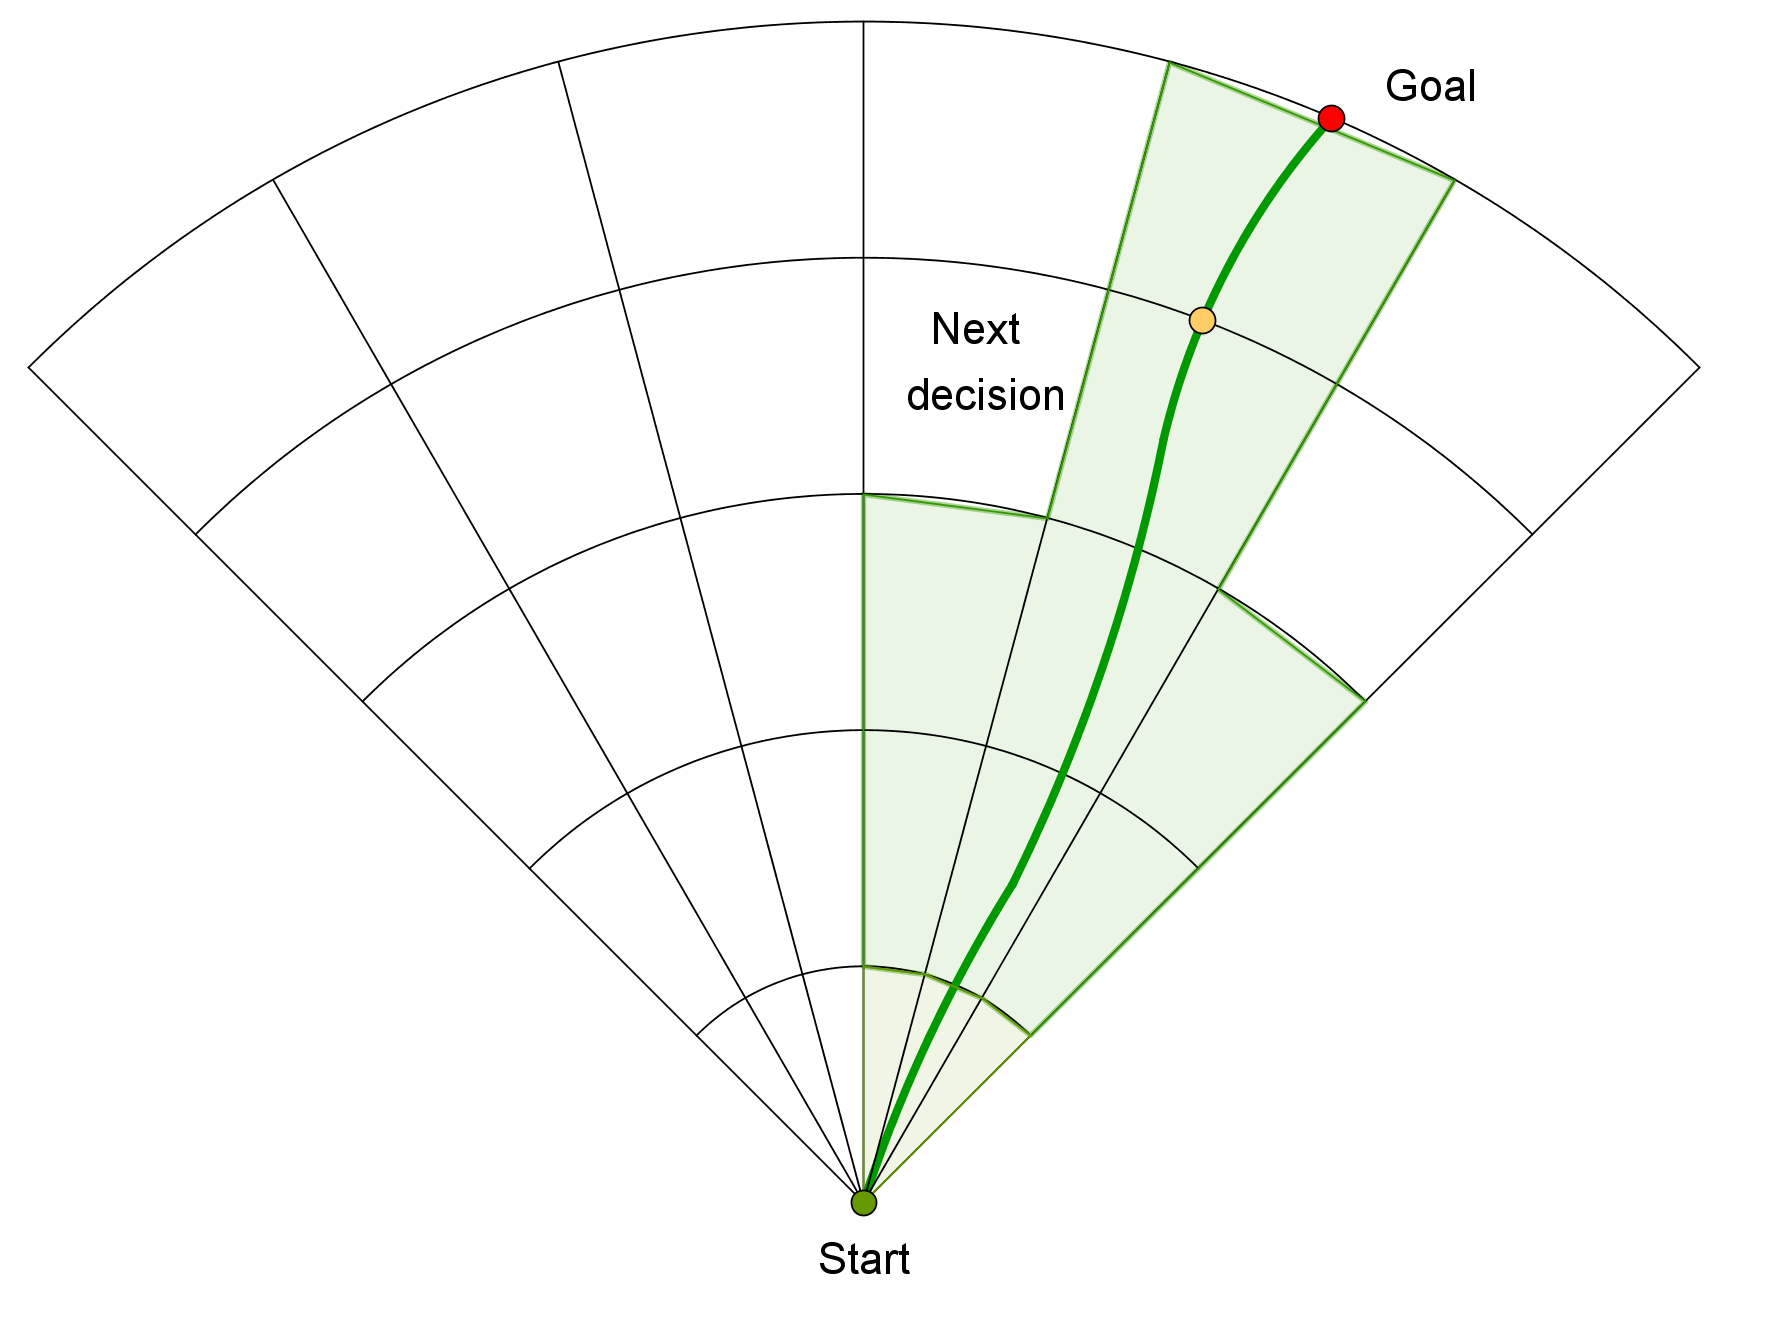
\includegraphics[width=0.9\linewidth]{\FIGDIR/CA005PathCalculation}
        \caption{Mission control run example.}
        \label{fig:missionControlRunExample}
    \end{subfigure}
    \begin{subfigure}{0.48\textwidth}
    	\centering
        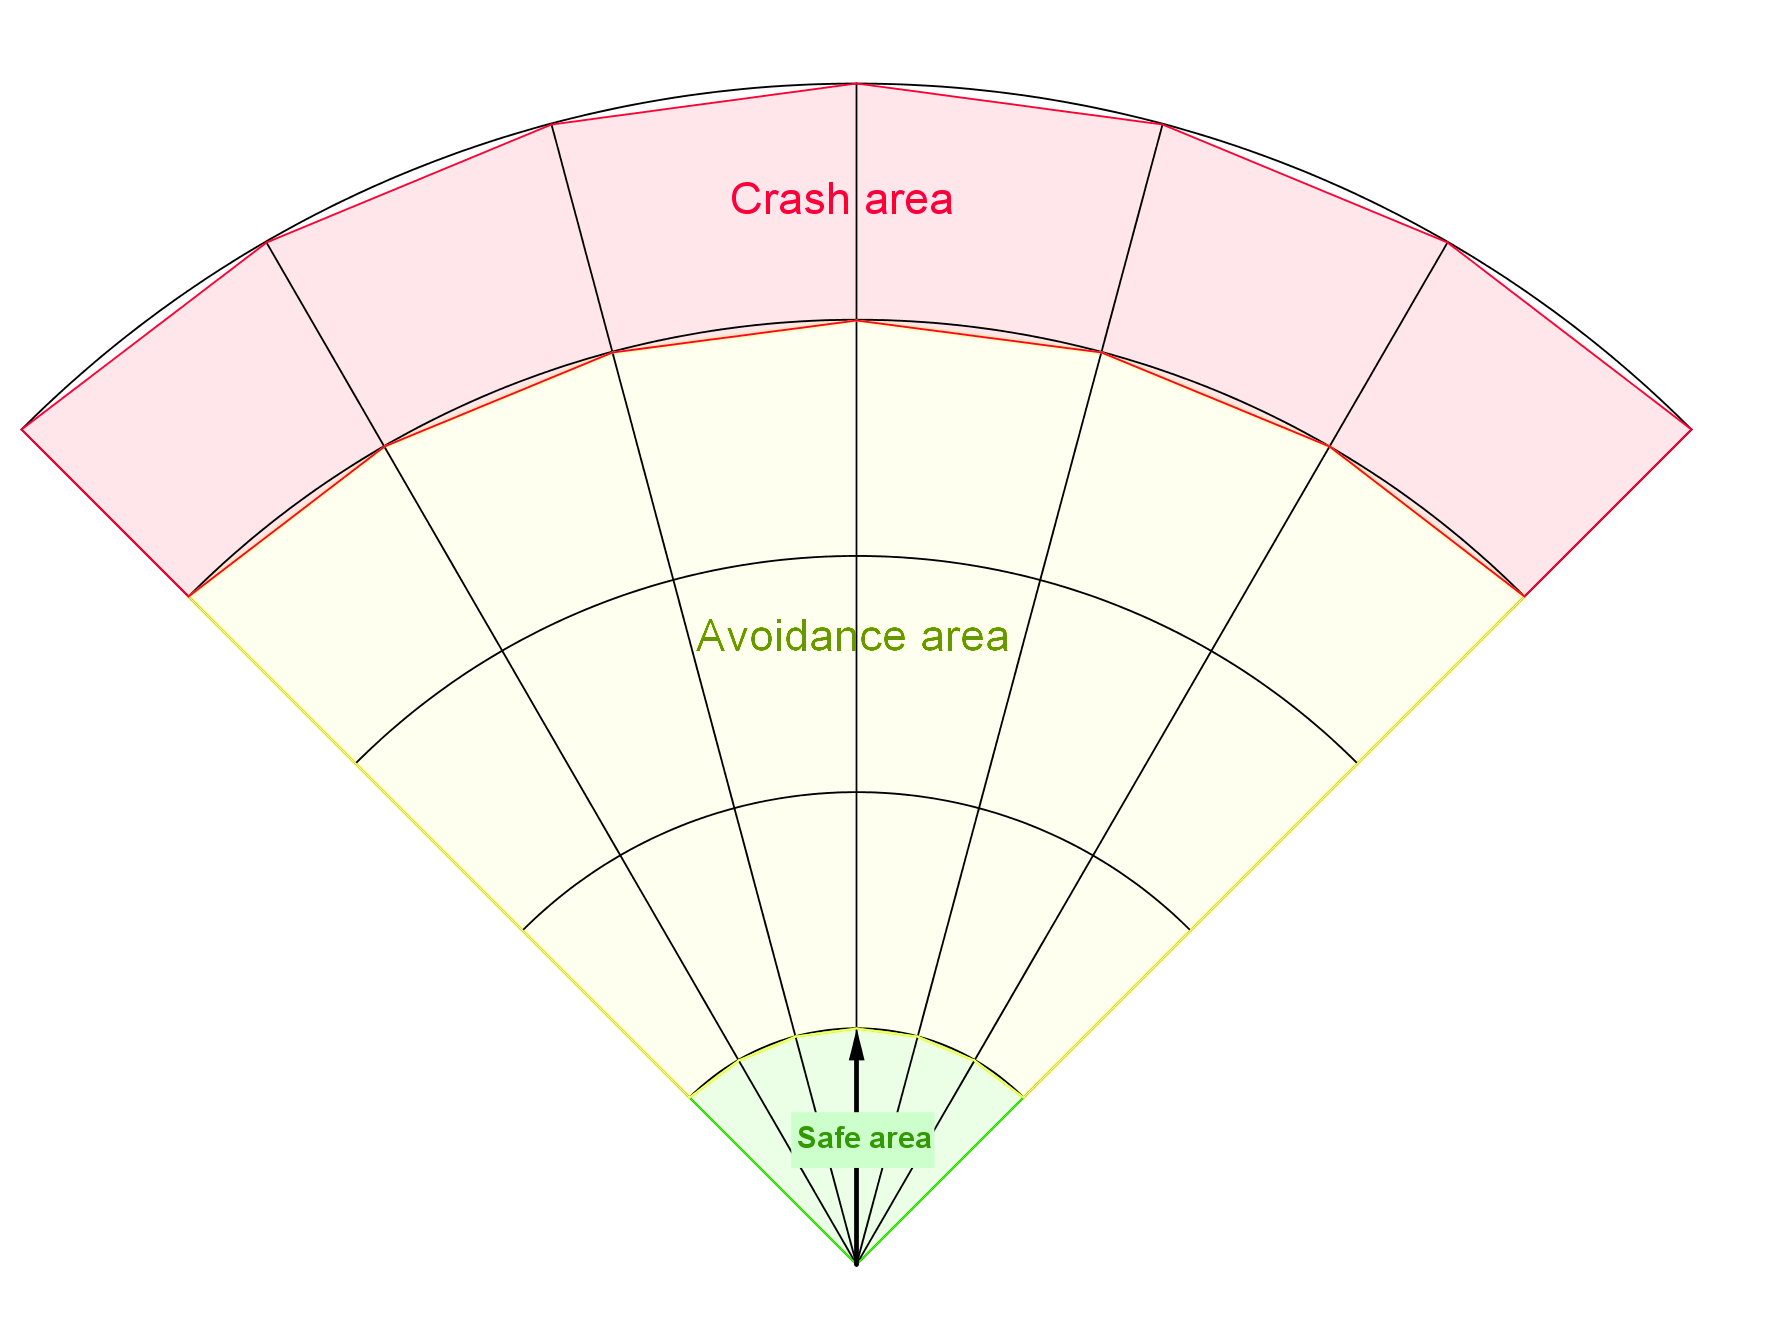
\includegraphics[width=0.9\linewidth]{\FIGDIR/CA006FieldOfViewZones} 
        \caption{Grid Zones.}
        \label{fig:gridZonesMissionControl}
    \end{subfigure}
    \caption{Definitions for \emph{Mission Control Run} (outer loop).}
    \label{fig:definitionsForMissionControlRun}
\end{figure}

\newpage
\noindent Joining \emph{Avoidance Grid Runs} (fig. \ref{fig:joiningMultipleAGRS})  example portrays \emph{Avoidance Grid Runs} invoked on various \emph{Decision Points} to achieve \emph{Navigation} functionality. The UAS (blue plane) is flying Mission (green numbered waypoints). The \emph{Avoidance Grid} boundary (black dashed line) for each \emph{Decision Point} (UAS position at time $t_i$). Following example of \emph{Navigation} (fig. \ref{fig:missionControlRunActivityDiagram}) run is shown:

\begin{enumerate}
    \item \emph{Mission Start} (fig. \ref{fig:missionExampleWithOAGR}) - UAS at the start of the mission have one \emph{Avoidance Grid} at its position to determine the \emph{Navigation Path} to \emph{Waypoint 2} (goal waypoint). The planned path (red line) is leading directly to \emph{Avoidance Grid} boundary (black dashed line).
    
    \item \emph{Mission End} (fig. \ref{fig:finishedMissionAGR}) - UAS have reached 
    \emph{last waypoint}. All \emph{Avoidance Grid} boundaries (black dashed line) for all \emph{runs} are drawn along flown trajectory. 
    
    \item \emph{Waypoint Reach} (fig. \ref{fig:waypointReachAGR}) - the \emph{waypoint} is inside \emph{Avoidance Grid}, the navigation path (red line) leads directly to \emph{goal waypoint}. (Excessive \emph{Avoidance Grid} boundaries are removed.)
    
    \item \emph{Next Waypoint} (fig. \ref{fig:newtWaypointAGR}) - the new \emph{Goal Waypoint} is selected, the UAS moves to new goal (invoking \emph{Avoidance Grid Runs} when necessary).
    
\end{enumerate}

\begin{figure}[H]
    \centering
    \begin{subfigure}{0.48\textwidth}
        \centering
        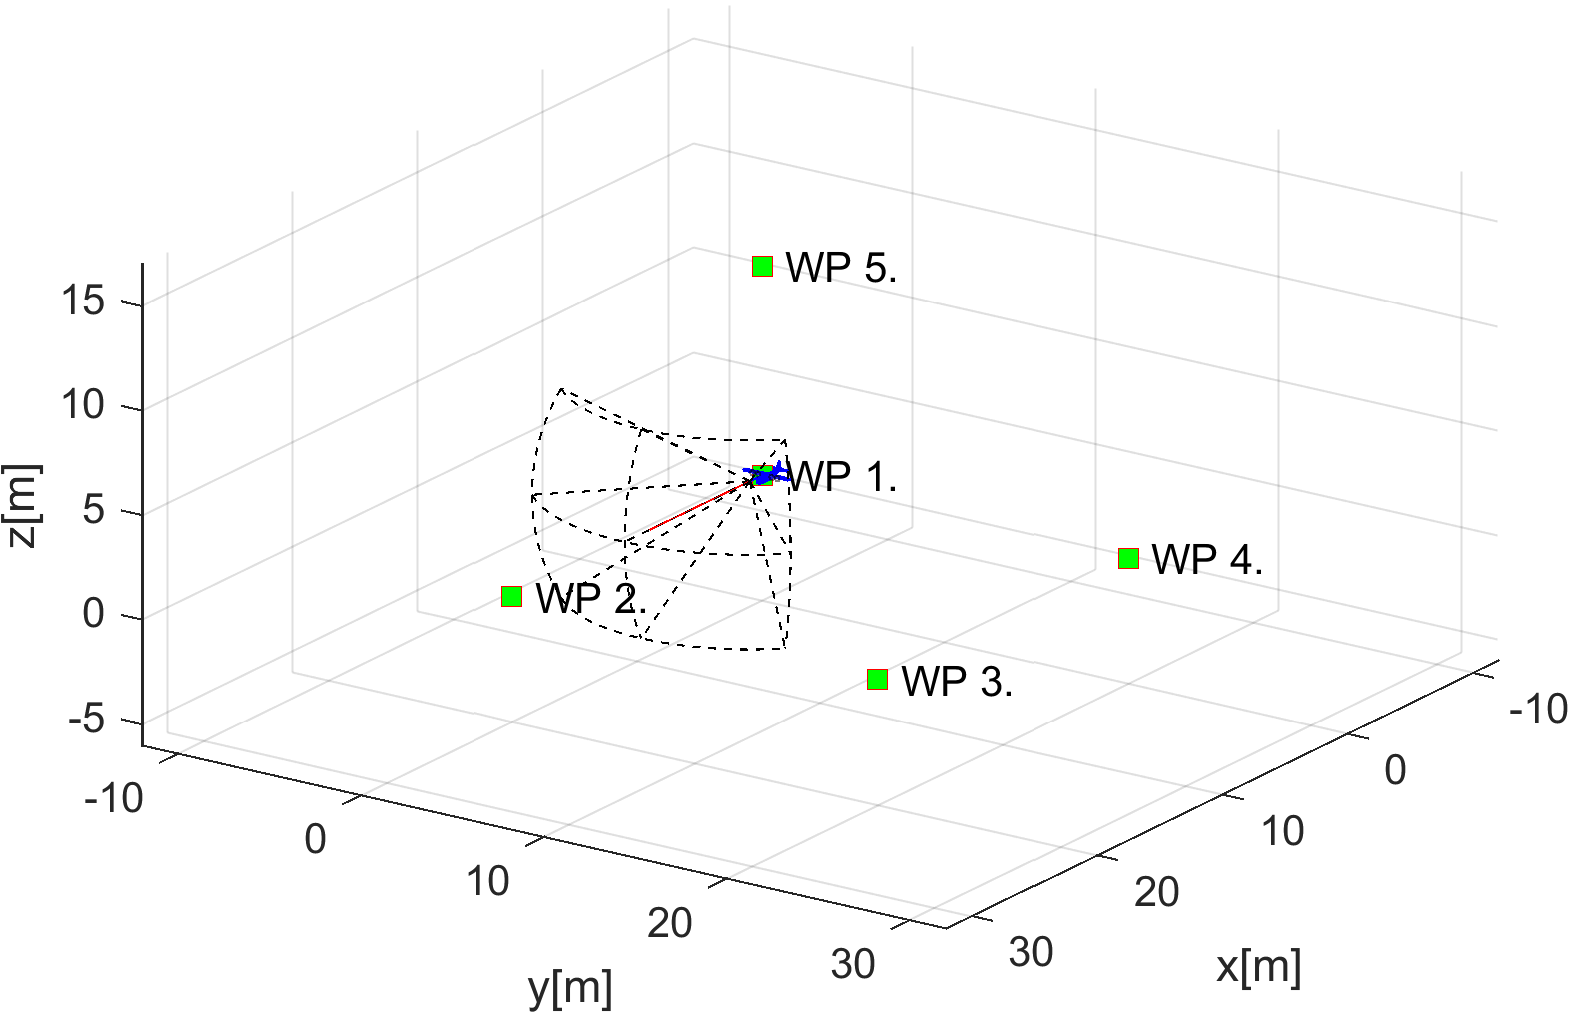
\includegraphics[width=0.9\linewidth]{\FIGDIR/TE042MissionExample}
        \caption{Mission start.}
        \label{fig:missionExampleWithOAGR}
    \end{subfigure}
    \begin{subfigure}{0.48\textwidth}
    	\centering
        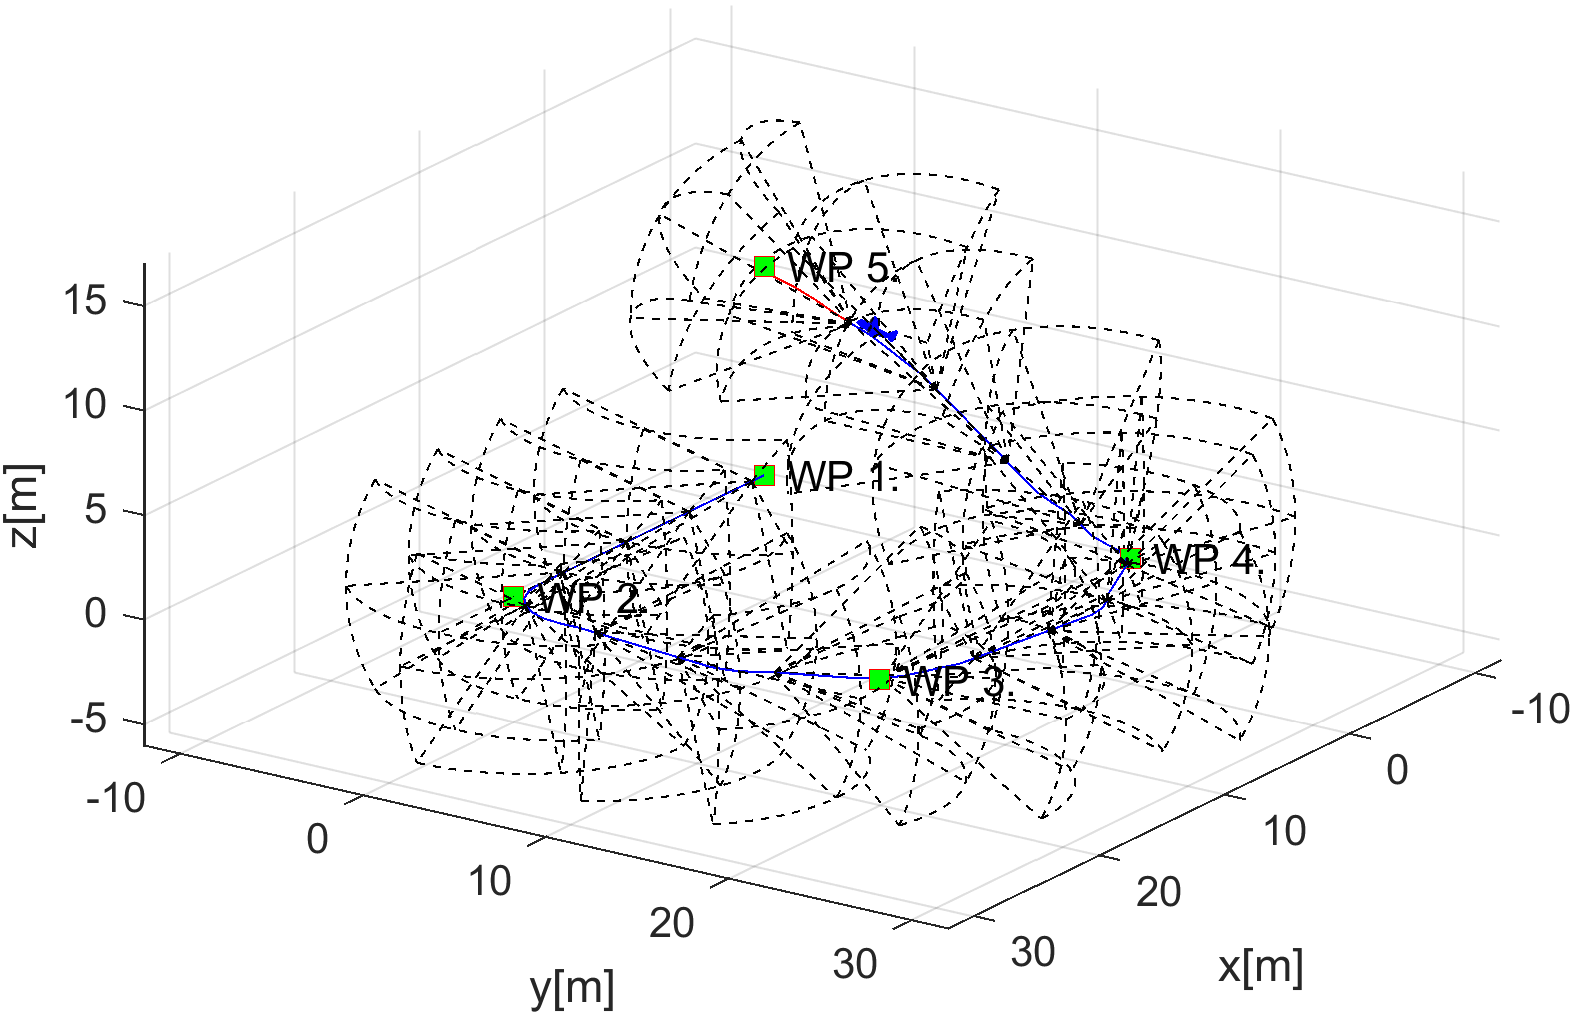
\includegraphics[width=0.9\linewidth]{\FIGDIR/TE043AllDecisionDecisionPoint} 
        \caption{Mission end.}
        \label{fig:finishedMissionAGR}
    \end{subfigure}
    \\
    \centering
    \begin{subfigure}{0.48\textwidth}
        \centering
        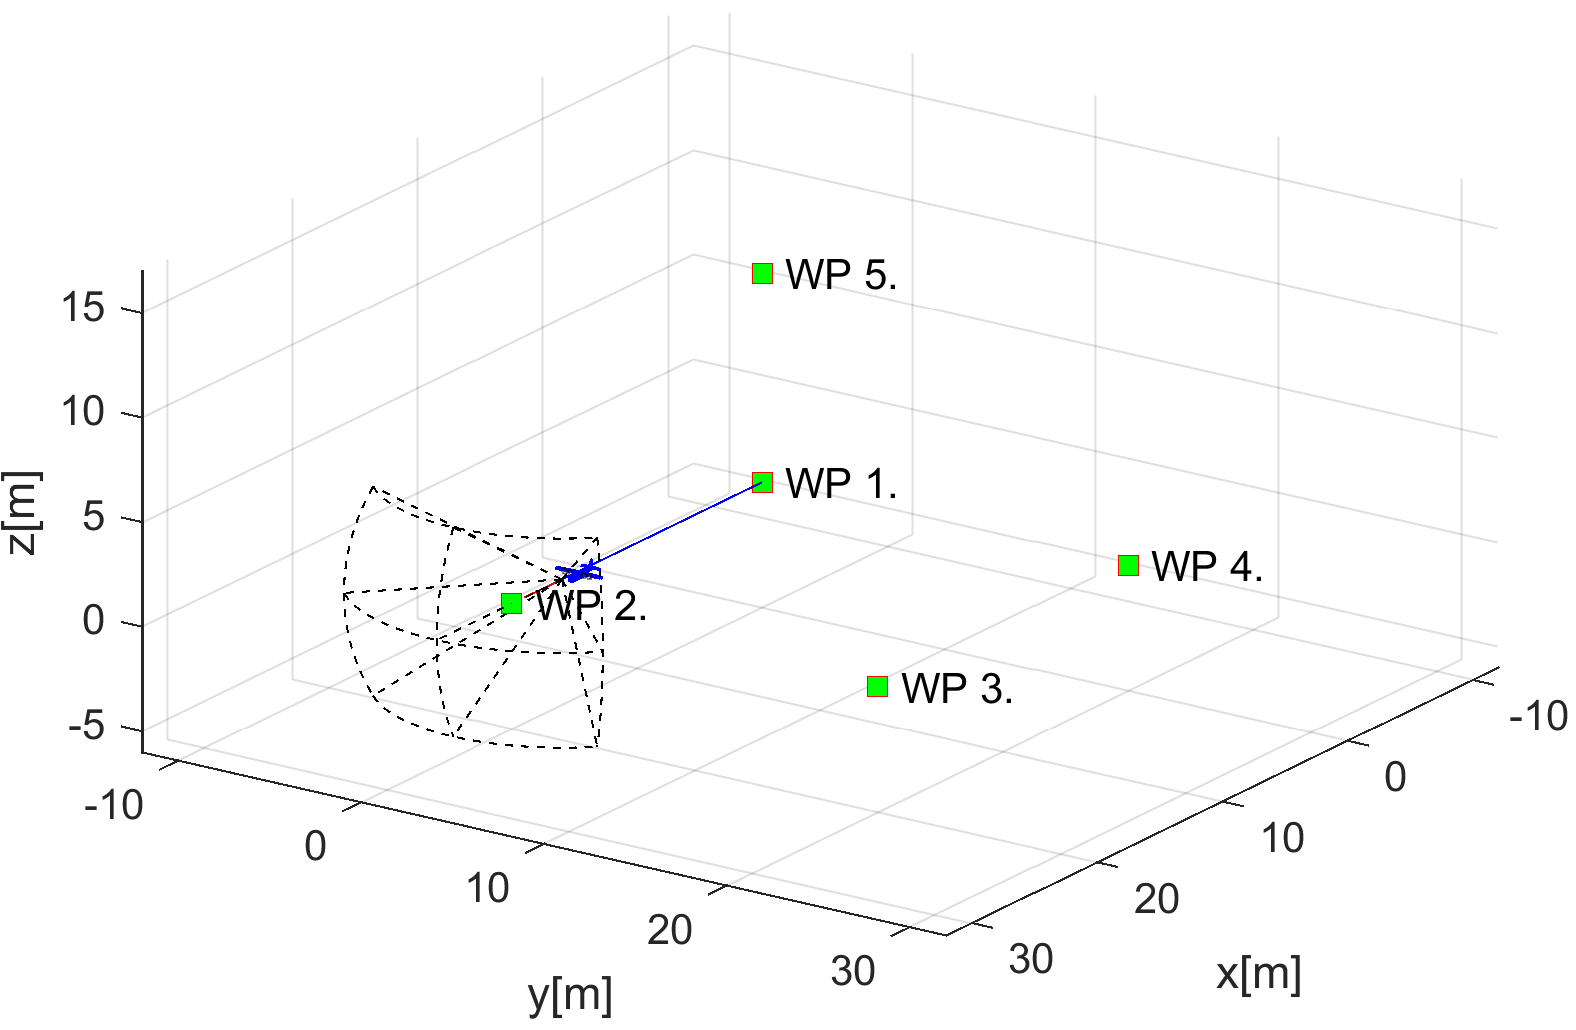
\includegraphics[width=0.9\linewidth]{\FIGDIR/TE044WaypointReach}
        \caption{Waypoint reach.}
        \label{fig:waypointReachAGR}
    \end{subfigure}
    \begin{subfigure}{0.48\textwidth}
    	\centering
        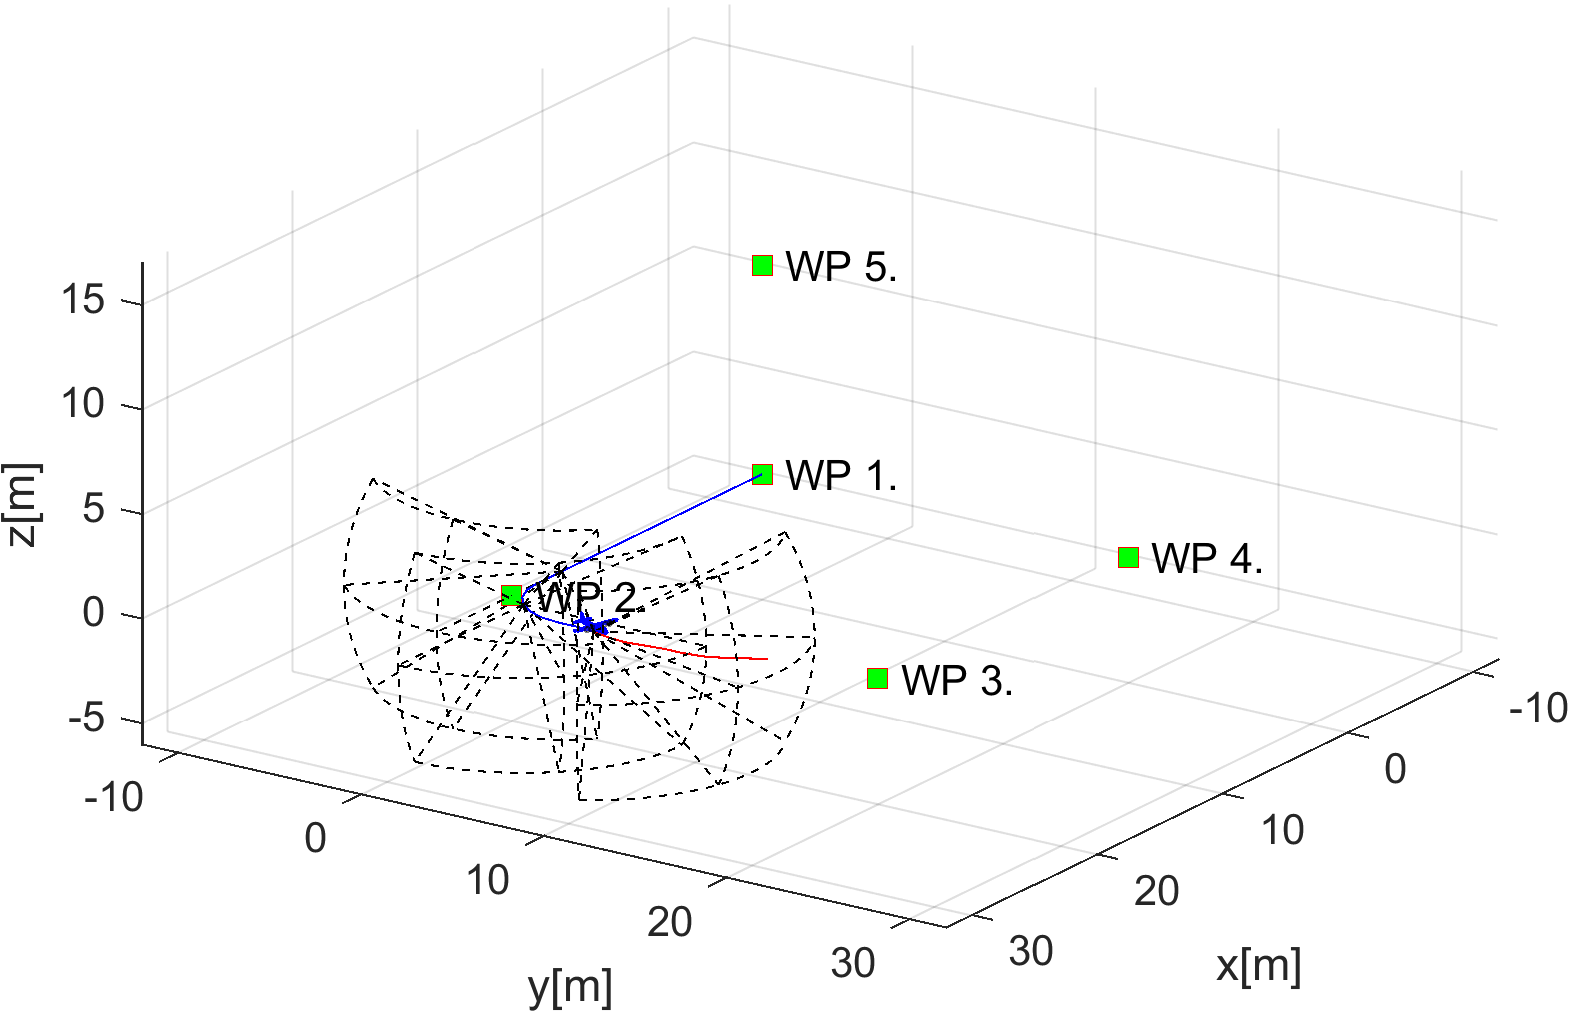
\includegraphics[width=0.9\linewidth]{\FIGDIR/TE045NewWaypointSetup} 
        \caption{Next waypoint.}
        \label{fig:newtWaypointAGR}
    \end{subfigure}
    \caption{Joining multiple \emph{Avoidance Grid Runs} for achieve Navigation.}
    \label{fig:joiningMultipleAGRS }
    
\end{figure}
    
    

\newpage
\paragraph{General Concept:}\footnote{Mission Control Run Function Implementation: \url{RuleEngine/MissionControl/MissionControl.m::runOnce(.)}} The \emph{General Concept} is taken from  \cite{sabatini2014navigation,Sabatini2014}, consisting from following main modules:
\begin{enumerate}
    \item \emph{Navigation Loop} - module responsible for \emph{Navigation} providing \emph{Goal Waypoint}.
    
    \item \emph{Data Fusion} (background in sec. \ref{s:sensorFusion}) - module responsible for \emph{Surveillance Data Feed}.
    
    \item \emph{Situation Assessment} - module responsible for \emph{UAS Safety Evaluation}. 
    
    \item \emph{Avoidance Run} (background in sec. \ref{s:aviudabceGridRun}) responsible for \emph{Avoidance Path} selection.    
\end{enumerate}


\begin{figure}[H]
    \centering
    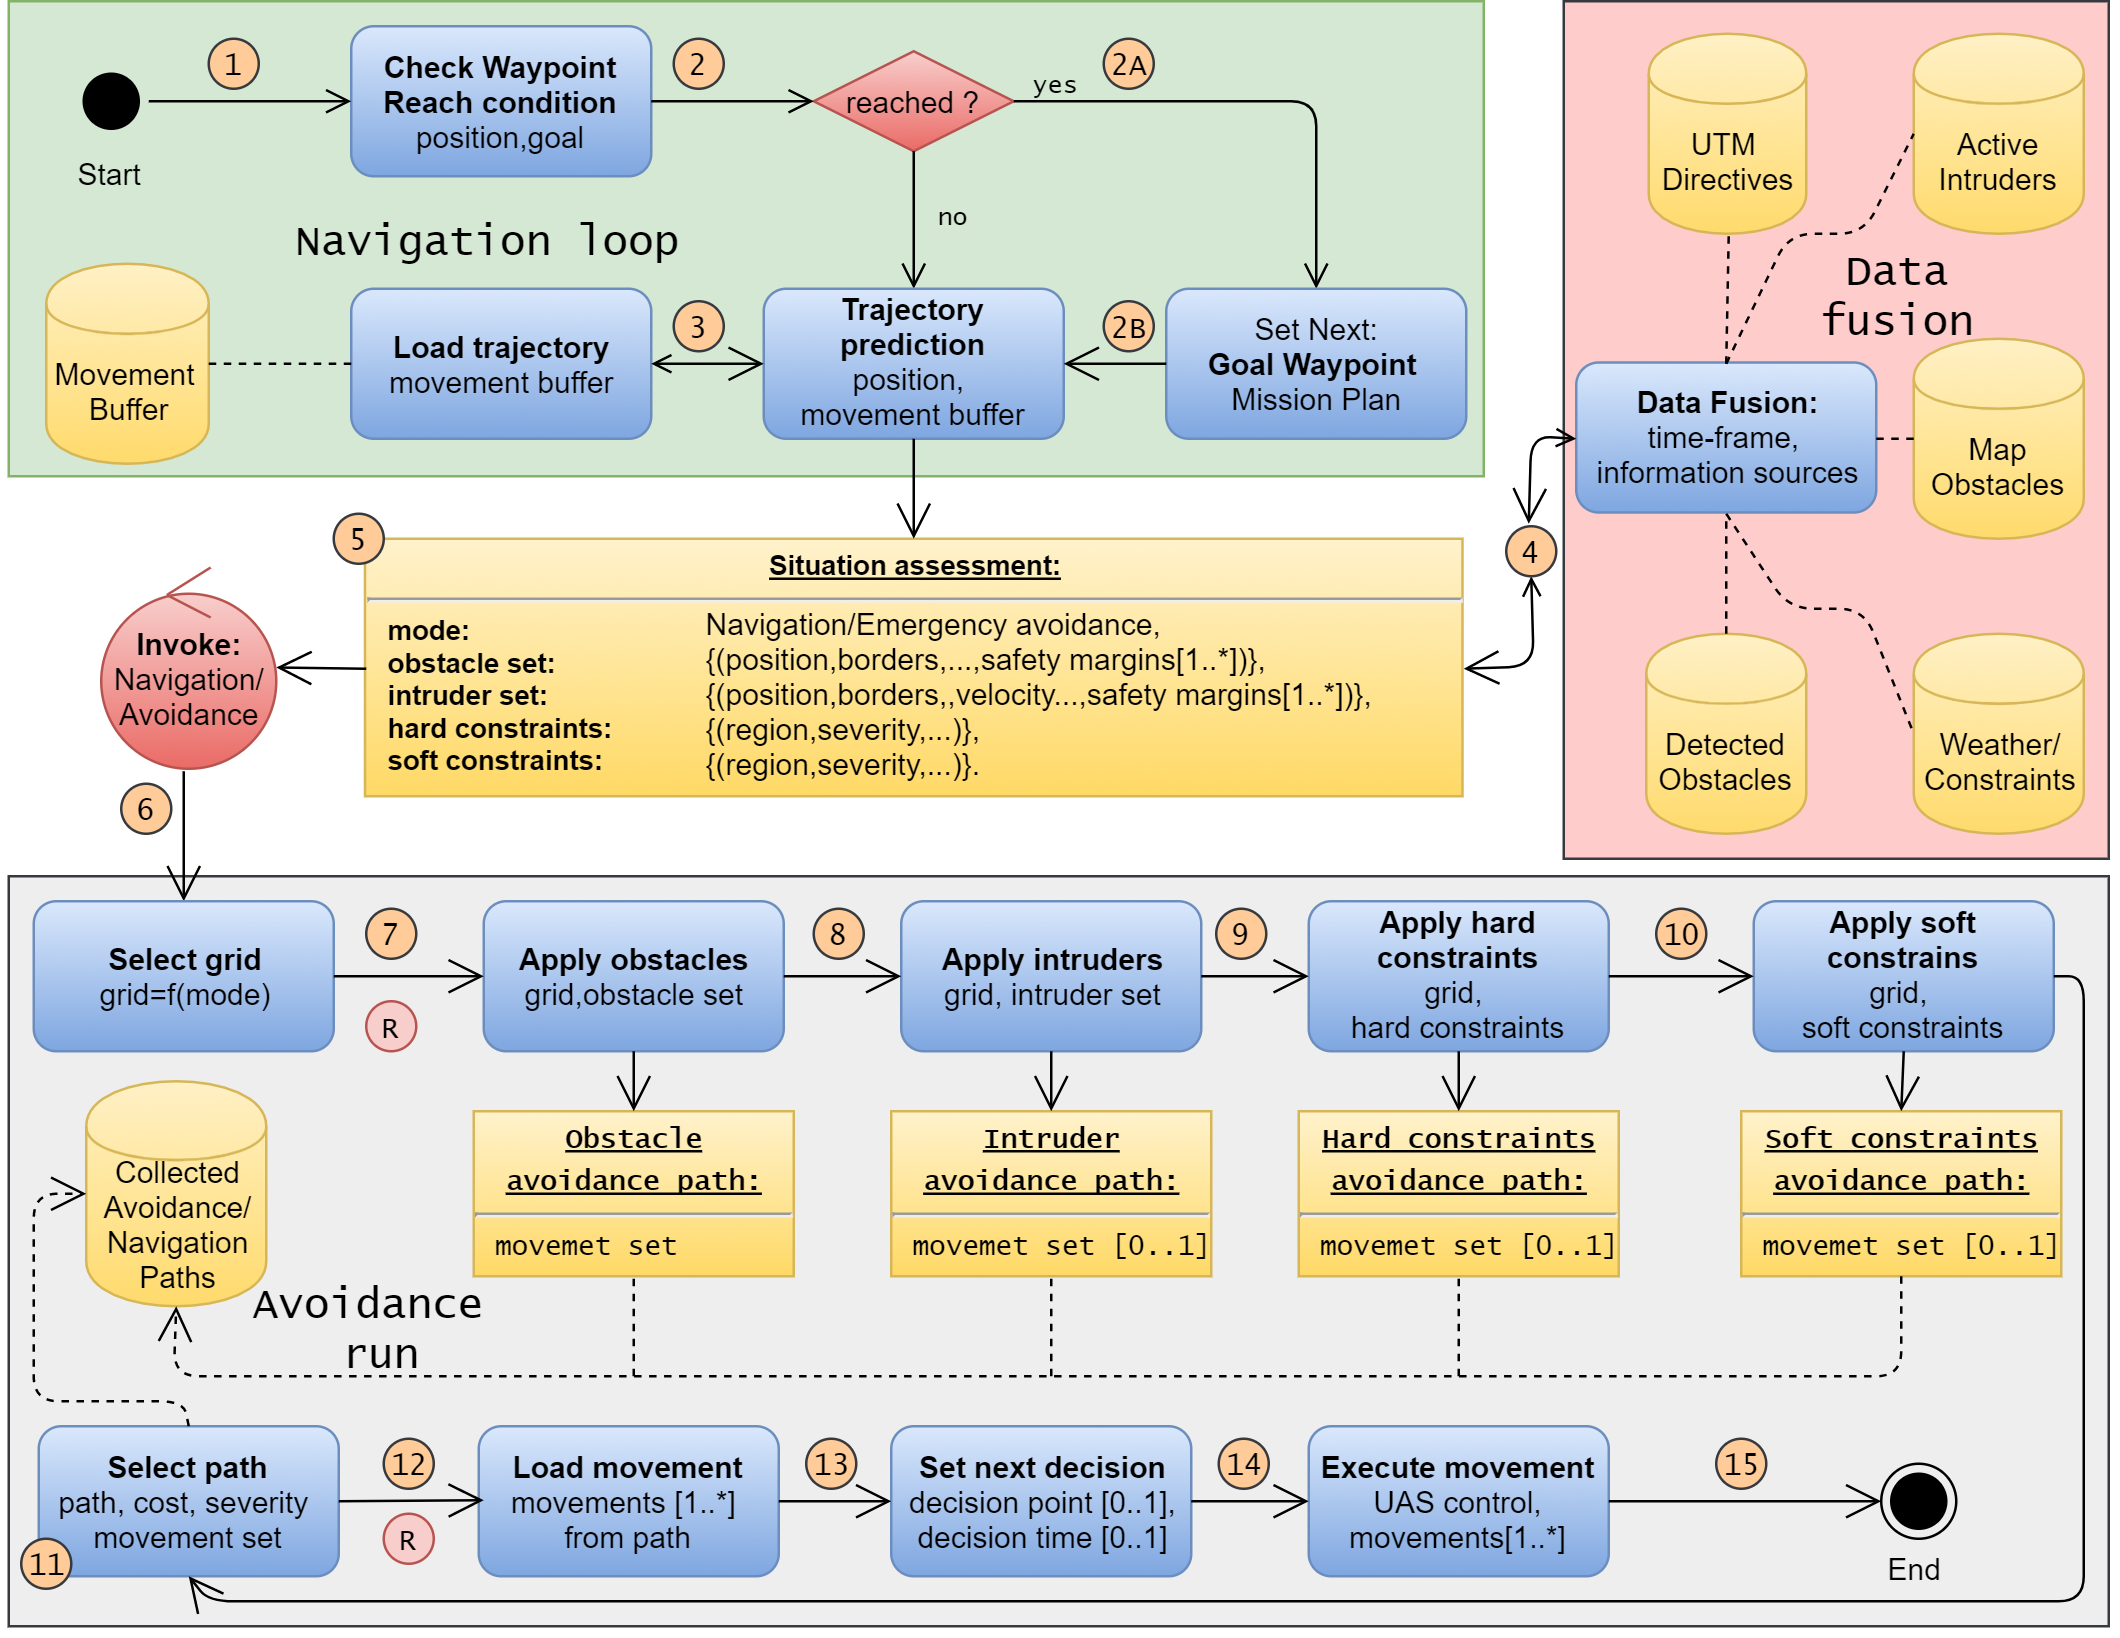
\includegraphics[width=\linewidth]{\FIGDIR/TE026AvoidanceAlgorithmMainLoopRun}
    \caption{Mission control run activity diagram.}
    \label{fig:missionControlRunActivityDiagram}
\end{figure}

\noindent The main changes to \emph{Navigation architecture} are given in \emph{Mission Control Run} activity diagram (fig. \ref{s:missionControlRunActivityDiagram}):

\begin{enumerate}
    \item \emph{Situation Assessment} - added event-based mode switching control. 
   
    \item \emph{Avoidance Run} - added hierarchical evaluation for \emph{Avoidance Path} selection. Prioritizing threat avoidance according to a type. 
\end{enumerate}

\newpage
\noindent The \emph{Operation Mode} is introduced, based on \emph{Situation assessment} and \emph{Triggering Events} one of following modes are selected in \emph{Avoidance Run}:

\begin{enumerate}
    \item \emph{Navigation Mode} - the \emph{UAS} is navigating trough \emph{Airspace} following \emph{cost effective patterns} and obeying \emph{Airspace Authority} (UTM). The \emph{Navigation Grid} is a instance of \emph{Avoidance Grid} (sec. \ref{s:AvoidanceGrid}) with initialized \emph{Navigation Reach Set} (ex. \emph{Harmonic Reach Set Approximation} (sec. \ref{s:harmonicReachSet})).
    
    \item \emph{Emergency Avoidance Mode} - the \emph{UAS} is \emph{threatened} by obstacle, intruder, hard constraint or \emph{soft constraint}, the \emph{UAS} is navigating trough \emph{Airspace} following \emph{safe avoidance patterns} and \emph{minimizing the impact} of possible damages. The \emph{Avoidance Grid} is term used for \emph{Emergency Avoidance Mode}. The \emph{Avoidance Reach Set Approximation} is initialized in \emph{Avoidance Grid} (ex. \emph{Chaotic Reach Set Approximation} (sec. \ref{s:chaoticReachSet}))
\end{enumerate}

\begin{note}
    Depending on \emph{Operation Mode} the pair of \emph{Avoidance Grid} and \emph{Reach Set} is selected in \emph{Avoidance Run} part.
    
    
    The \emph{Navigation Grid} and \emph{Avoidance Grid} shares the space segmentation pattern, therefore the \emph{Data Fusion} (sec. \ref{s:sensorFusion}) needs to be evaluated only once for both grids. 
\end{note}



\paragraph{Decision Time Frame ($[t_i,t_{i+1}[$):} The \emph{Mission Control Run} is executed for \emph{Decision Time Frame} bounded to the \emph{period} of the \emph{UAS executed movement} (fig. \ref{fig:AvoidanceFrameworkConceptNew}).

The \emph{UAS System} (sec. \ref{s:UASNonlinearModel}) controlled by \emph{Movement Automaton Implementation} (sec. \ref{s:movementAutomatonDefinition}) \emph{Planned Movements} can be changed at any time. The real impact on control is shown after the \emph{actual movement} is executed. 

\begin{note}
    For our \emph{Movement Automaton Implementation} movements the average \emph{movement duration} is \emph{1/velocity second} (tab. \ref{tab:movements1}, \ref{tab:movements2}).
\end{note}

The \emph{Decisions} are made based on \emph{system} state in \emph{current} time-frame started at $t_i$ for \emph{next} time frame starting at $t_{i+1}$.

\begin{note}
    Because the \emph{Decision Delay} is crucial in \emph{Avoidance System} it is beneficial to have \emph{short time movements}. On the other hands, the \emph{length and duration  of movements} is impacting \emph{Reach Set Complexity}. The proper construction of movement automaton is greatly impacting overall \emph{approach performance}.
\end{note}

\paragraph{Initialization:} The \emph{UAS} is going to solve a problem for \emph{Rules of the Air} (eq. \ref{eq:rulesOfTheAir}). Using control scheme (fig. \ref{fig:AvoidanceFrameworkConceptNew}) with given \emph{Sensors}:

\begin{equation}
    Sensors = \{LiDAR,ADS-B\}
\end{equation}

\noindent The sensors obstacle assessment into avoidance grid is outlined for static obstacles in (sec. \ref{s:staticObstacles}) and for moving obstacles in (sec. \ref{s:intruders}.)

The \emph{Data Fusion Procedure} is given as follow:
\begin{equation}
    DataFusion = \{Rating Based Data Fusion \quad (sec. \ref{s:sensorFusion})\}
\end{equation}

Then the \emph{UAS system} (sec. \ref{s:UASNonlinearModel}) with \emph{Movement Automaton Implementation} (sec. \ref{s:movementAutomatonDefinition}) with empty movement buffer:

\begin{equation}
    Movement Buffer = \{\}
\end{equation}

The \emph{Avoidance Grids} for both \emph{Operation Modes} are created with \emph{identical space segmentation}. The \emph{Reach Set Approximations} are loaded based on initial \emph{UAS State} at decision time $0$. The \emph{Reach Set Approximation} is always selected based on \emph{UAS System State}. The initial \emph{Operation Mode} is set up as \emph{Navigation}. The initialization is summarized like follow:

\begin{equation}
    \begin{aligned}
    Avoidance Grid(0) &= \{UAS.position(0),AvoidanceReachSet(UAS.ReachSet)\}\\
    Navigation Grid (0) &= \{UAS.position(0), NavigationReachSet(UAS.ReachSet)\}\\
    Operation Mode &= Navigation
    \end{aligned}
\end{equation}

The \emph{Mission} is set up as a set of \emph{ordered waypoints}. The \emph{initial goal waypoint} is \emph{first waypoint}. The initialization is summarized like follow:

\begin{equation}
    \begin{aligned}
    Mission &= \{Waypoint_1 \dots  Waypoint_n\}\\
    Goal Waypoint &= Mission.waypoint_1\\
    Last Waypoint &= Mission.waypoint_n\\
    \end{aligned}
\end{equation}

The \emph{actual threats} are set as empty sets for \emph{decision time} $t_i=0$:
\begin{equation}
    \begin{aligned}
    obstacles &= \{\}, intruders = \{\}, hard Constraints = \{\}, soft Constraints = \{\}\\
    \end{aligned}
\end{equation}



\paragraph{Navigation Loop (1\textsuperscript{st}-3\textsuperscript{rd} step):} The purpose of \emph{Navigation Loop} is to select proper \emph{Goal Waypoint} from \emph{Mission} (sec. \ref{s:mission}). If \emph{last waypoint} have been reached the \emph{Landing Procedure} will be initiated and \emph{Mission Control Run} Ends.

First start with definition of \emph{waypoint reach condition} (def. \ref{def:waypointReachCondition}) and \emph{Unreachable waypoint} (def. \ref{def:unreachable Waypoint}).

\begin{definition}{Waypoint Reach Condition}\label{def:waypointReachCondition} for \emph{current} decision time $t_i$ for \emph{UAS} position and current \emph{Goal Waypoint} is satisfied only if:

\begin{multline}\label{eq:waypointReachCondition}
    distance(UAS.position(t_i),GoalWaypoint(t_i)) \\\le \\2 \times \max \left\{length(movement):\forall movement\in MovementSet\right\}
\end{multline}

    \begin{note}
        The movements in our solution have \emph{uniform length} of \emph{1 m} (tab. \ref{tab:movements1}, \ref{tab:movements2}), therefore the waypoint reach condition is satisfied when \emph{distance to goal waypoint} is lesser than 2 m. The maximal movement length has impact on \emph{navigation/avoidance} precision.
    \end{note}
\end{definition}

\begin{definition}{Unreachable Waypoint}\label{def:unreachable Waypoint}. The \emph{Goal Waypoint} is evaluated as unreachable in decision time $t_i$ when \emph{Avoidance Grid Run} (alg. \ref{alg:FindBestPathAvoidanceGrid}) can not find the \emph{navigation/avoidance path} leading to it.

\noindent Formally: The \emph{Avoidance/Navigation Grid} has range defined as \emph{final layer distance}. When the \emph{Goal Waypoint} is in  \emph{range} of \emph{Grid}:

\begin{equation}
    Grid(t_i).range \ge distance(UAS.position(t_i),GoalWaypoint(t_i))
\end{equation}

\noindent and following condition is satisfied:

\begin{multline}\label{eq:unreachableWaypoint}
    \forall cell_{i,j,k}\in Grid(t_i) \not\exists cell_{i,j,k}. Reachable == true \wedge\dots  \\\dots\wedge distance(cell_{i,j,k}, Goal Waypoint(t_i)) \le\dots \\ \dots\le 2 \times \max \left\{length(movement):\forall movement\in MovementSet\right\}
\end{multline}

\noindent The \emph{Goal Waypoint} is unreachable.

\end{definition}

Then the \emph{Navigation Loop} is invoked  every \emph{decision time} $t_i$, \emph{Mission Control Run} (fig. \ref{fig:missionControlRunActivityDiagram}), it is described as sequence of following steps:

\begin{itemize}
    \item[\textbf{1\textsuperscript{st}}] \textbf{Check Waypoint Reach Condition} - the \emph{UAS position} for given \emph{time frame} $t_i$ is checked under condition (eq. \ref{eq:waypointReachCondition}).  If condition is met continue with 2\textsuperscript{nd} step otherwise continue with 3\textsuperscript{rd} step.

    \item[\textbf{2\textsuperscript{nd}}] \textbf{Set Next Waypoint} - until following condition is met:
    \begin{equation*}
        Goal Waypoint == Last Waypoint    
    \end{equation*}
    Set next goal waypoint like follow:
    \begin{equation*}
        Goal Waypoint = Mission.get Next Waypoint()
    \end{equation*}
    Otherwise enforce \emph{Landing sequence} (Out of Scope).
        
    \item[\textbf{3\textsuperscript{rd}}] \textbf{Trajectory Prediction} - the \emph{Movement Buffer} is loaded with planned movements from \emph{Movement Automaton}. The \emph{future trajectory} is predicted according to (eq. \ref{ourTrajectoryImplementation}):
    \begin{multline*}
        Predicted Trajectory = \\Trajectory(state=UAS.state(t_i),buffer=future Movements)
    \end{multline*}
\end{itemize}

\noindent The \emph{Predicted Trajectory} is used in 5\textsuperscript{th} step \emph{Situation Assessment}.

\paragraph{Data Fusion (4\textsuperscript{th} step)} The \emph{Data Fusion} (sec. \ref{s:sensorFusion}) in this context is \emph{Threat Sets} preparation for \emph{Avoidance Run}. It is depending on values of \emph{Boolean values} defined in (tab. \ref{tab:defuzificationRatings}) for \emph{threat} classification.

\begin{note}
    Avoidance Grid`s Data fusion (sec. \ref{s:sensorFusion}) is run in 7\textsuperscript{th}- 10\textsuperscript{th} step (fig. \ref{fig:missionControlRunActivityDiagram}). 
\end{note}

The \emph{static obstacles} source is from \emph{LiDAR} scan received at least at beginning of current \emph{decision frame} $t_i$:

\begin{equation*}
        obstacles=LiDAR.scan(UAS.position(t_i))
\end{equation*}

The \emph{intruders} source are valid \emph{active intruders notifications} received from ADS-B In positioned to \emph{future expected positions} at \emph{decision time} $t_{i+1}$:

\begin{equation*}
        intruders=ADS-B.get Active Intruders(t_{i+1})
\end{equation*}

\begin{note}
    The \emph{Intruders} needs to be predicted for the next decision time-frame starting at time $t_{i+1}$ Due their mobility.
\end{note}

The \emph{hard/soft constraints} are obtained from \emph{Information Sources} and the area of next decision time $t_{i+1}$ \emph{Avoidance Frame} is used as space parameter in search. The sets of hard and soft constraints are obtained in following manner:

\begin{equation*}
    hard Constraints= Information Sources.fuse(Avoidance Grid(t_{i+1}))
\end{equation*}

\begin{equation*}        
        soft Constraints=Information Sources.fuse(Avoidance Grid(t_{i+1}))
\end{equation*}

The results of \emph{Data Fusion} threats set preparation are used in next step.


\paragraph{Invoke Navigation/Avoidance based on Situation Assessment (5\textsuperscript{th}-6\textsuperscript{th} step):} The \emph{deciding events} depending on \emph{Trajectory Prediction} ($3^{rd}$ step) and \emph{Data Fusion} ($4^{th}$ step) (fig. \ref{fig:missionControlRunActivityDiagram}) are following:

\begin{enumerate}
    \item \emph{General Events} are \emph{triggered} regardless \emph{Operation Mode}. They are considered after \emph{specific mode events} are handled and \emph{Navigation/Avoidance Grid} is selected:
    \begin{enumerate}[a.]
        \item \emph{Empty Movement Buffer} ($Movement Buffer = \varnothing$) - if there is no movement in \emph{Movement buffer} to be executed (from 3\textsuperscript{rd} step: Load Trajectory), the \emph{Avoidance Run} is enforced to run with \emph{Navigation/Avoidance Reach Set Approximation} to generate new path.
        
        \item \emph{Waypoint Reached} (2\textsuperscript{nd} step) - the \emph{Navigation Loop} run is forced to set goal \emph{Goal Waypoint}. If \emph{last waypoint} from \emph{Mission} (sec. \ref{s:mission}) the \emph{Landing Procedure} is enforced.
        
        \item \emph{Waypoint Unreachable} - this type of event is very situations based. The \emph{Waypoint Reachibility} (assumption. \ref{ass:reachableWaypoints}) has not been relaxed, therefore this event is not properly handled in approach. The \emph{implementation} considers \emph{selecting next waypoint in mission} as a goal waypoint of \emph{first waypoint} if \emph{unreached/unreachable waypoints} are exhausted. 
    \end{enumerate}
    
    \item \emph{Navigation Mode Events} are triggered if \emph{Operation Mode} is set as \emph{Navigation}:
    \begin{enumerate}[a.]
        \item \emph{Empty Navigation Grid} ($|threats| = 0$) - if \emph{movement buffer} contains at least one \emph{movement}, the \emph{Avoidance Run} is omitted. The \emph{Operation Mode} stays in \emph{Navigation Mode}.
        
        \item \emph{Collision Case Resolution} ($|ActiveCollisionCases| > 0$) - there is new/active \emph{Collision Case} (sec. \ref{sec:collisionCase}), the \emph{Navigation Reach Set Approximation} trajectories will be constrained according to  active \emph{Collision Case(s)} requirements. If there exists at least one \emph{Reachable} avoidance path, the \emph{Operation Mode} will remain \emph{Navigation}. If there is no  \emph{Reachable} avoidance path, the \emph{Operation Mode} switches to \emph{Emergency Avoidance}.
        
        \item \emph{Static Obstacle Detection} ($LiDAR.Hits > threshold$) - if \emph{static obstacle set} contains at least one \emph{detected obstacle} (sec. \ref{s:detectedObstacles}) intersecting with \emph{Navigation  grid} the \emph{Operation Mode} will be \emph{switched} to \emph{Emergency Avoidance Mode}.
        
        \item \emph{Intruder Detection} ($intruders> 0$) - if \emph{active intruders set} contains at least one \emph{intruder} which expected impact area (intersection models (sec. \ref{s:intruderBehaviourPrediction})) \emph{Navigation  grid} the \emph{Operation Mode} will be \emph{switched} to \emph{Emergency Avoidance Mode}.
        
        \item \emph{Hard or Soft Constraint Occurrence} ($|hard Constraints|$ $>$ $0$ $\vee$ $|soft Constraints|$ $>$ $0$) - if \emph{hard/soft constraint set} contains at least one \emph{constraints} which intersects (static constraints (sec. \ref{s:virtualConstraints}), moving constraints (sec. \ref{s:MovingVirtualConstraints})) \emph{Navigation  grid} the \emph{Operation Mode} will be \emph{switched} to \emph{Emergency Avoidance Mode}.
    \end{enumerate}
    
    \item \emph{Emergency Avoidance Events} are triggered if \emph{Operation Mode} is set as \emph{Emergency Avoidance}:
    \begin{enumerate}[a.]
        \item \emph{Empty Avoidance Grid} ($|threats| = 0$) - if there is no \emph{detectable} threat, the remainder of \emph{avoidance path} is removed from \emph{Movement Buffer}. The \emph{Operation Mode} is switched to \emph{Navigation} and new \emph{navigation path} is selected. 
    \end{enumerate}
\end{enumerate}



\begin{itemize}
    \item[\textbf{5\textsuperscript{th}}] \textbf{Situation Assessment} - if there is any flag raised by \emph{Event Triggers}, there is an \emph{avoidance situation}.
    
    The \emph{Event Triggers} describe complex \emph{Operation Mode} switching. The simplified principle is following: \emph{If UAS is in Emergency Avoidance Mode Always Invoke Avoidance Run. If UAS is in Navigation Mode Invoke Only if Necessary}.
    
    If there was event trigger continue with 7\textsuperscript{th} step, otherwise wait for \emph{next decision time} $t_{i+1}$, execute movement and continue with 1\textsuperscript{st} step.
    
    \item[\textbf{6\textsuperscript{th}}] \textbf{Invoke Navigation/Avoidance} depending on the \emph{Operation Mode} the \emph{Reach Set/Grid} pair is selected. The future $state(t_{i+1})$ in next decision frame $t_{i+1}$ is necessary for Grid/Reach Set initialization. The \emph{next decision frame initial state} is obtained by \emph{prediction}:
    
    \begin{equation*}
        state(t_{i+1}) =  Trajectory(state(t_i),current Movement)
    \end{equation*}
    
    The \emph{Reach Set Approximation} is loaded based on \emph{mode} and $state(t_{i+1})$. The \emph{Grid} is initialized as $Free(t_{i+1})$ (eq. \ref{eq:freeDataFusion}) for all cells.
\end{itemize}



\paragraph{Avoidance Run (7\textsuperscript{th}-15\textsuperscript{th} step):} The \emph{Avoidance Run} goal is to obtain \emph{Path} represented as \emph{Trajectory}(state($t_{+1}$,MovementBuffer)) (eq. \ref{eq:ourTrajectoryImplementation}) from \emph{Navigation/Avoidance Grid} and associated \emph{Navigation/Avoidance Reach Set Approximation}.

If the \emph{Operation Mode} is set as \emph{Navigation Mode} the algorithm continues with 11\textsuperscript{th} step. Otherwise the \emph{Avoidance Grid Space Assessment} is run multiple times to obtain $Reachable(t_{i+1})$ (eq. \ref{eq:ReachableDataFusion}). The \emph{Threat Data} obtained from 4\textsuperscript{th} step are used. 

\begin{itemize}
    
    \item[\textbf{7\textsuperscript{th}}] \textbf{Apply Obstacles} - The \emph{Space assessment} (tab. \ref{tab:defuzificationRatings}) for \emph{Avoidance Grid} is calculated  with following threat modification:
    
    \begin{equation*}
        intruders = \varnothing, soft Constraints = \varnothing, hard Constraints = \varnothing
    \end{equation*}
    
    The \emph{Find Best Path} (alg. \ref{alg:FindBestPathAvoidanceGrid}) is applied, the resulting \emph{avoidance path} is labeled as \emph{Obstacle Avoidance Path}.
    
    \item[\textbf{8\textsuperscript{th}}] \textbf{Apply Intruders} - The \emph{Space assessment} (tab. \ref{tab:defuzificationRatings}) for \emph{Avoidance Grid} is calculated  with following threat modification:
    
    \begin{equation*}
        soft Constraints = \varnothing, hard Constraints = \varnothing
    \end{equation*}
    
    The \emph{Find Best Path} (alg. \ref{alg:FindBestPathAvoidanceGrid}) is applied, the resulting \emph{avoidance path} is labeled as \emph{Intruders Avoidance Path}.
    
    \item[\textbf{9\textsuperscript{th}}] \textbf{Apply Hard Constraints} - The \emph{Space assessment} (tab. \ref{tab:defuzificationRatings}) for \emph{Avoidance Grid} is calculated  with following threat modification:
    
    \begin{equation*}
        hard Constraints = \varnothing
    \end{equation*}
    
    The \emph{Find Best Path} (alg. \ref{alg:FindBestPathAvoidanceGrid}) is applied, the resulting \emph{avoidance path} is labeled as \emph{Hard Constraint Avoidance Path}.
    
    \item[\textbf{10\textsuperscript{th}}] \textbf{Apply Soft Constraints} - The \emph{Space assessment} (tab. \ref{tab:defuzificationRatings}) for \emph{Avoidance Grid} is calculated  without any modification.
    
    The \emph{Find Best Path} (alg. \ref{alg:FindBestPathAvoidanceGrid}) is applied, the resulting \emph{avoidance path} is labeled as \emph{Soft Constraints Avoidance Path}.
    
    \begin{note}
        The 7\textsuperscript{th} to 10\textsuperscript{th} steps are code-optimized for efficient calculation.
    \end{note}
    
    \item[\textbf{11\textsuperscript{th}}] \textbf{Select Path} -  based on \emph{Operation Mode} the \emph{Navigation/Avoidance Path} is selected.
    
    The \emph{Navigation Path} for \emph{Navigation Mode} is selected by standard \emph{Find Best Path} (alg. \ref{alg:FindBestPathAvoidanceGrid}) procedure. The \emph{Navigation Reach Set Approximation} can be constrained by \emph{Rule Engine} (fig. \ref{fig:RuleEngineInstanceLevels}).
    
    The \emph{Avoidance Path} for \emph{Emergency Avoidance Mode} is selected from \emph{Collected Avoidance Paths} with following priority:
    \begin{itemize}
        \item[1.] \emph{Soft Constraints Avoidance Path} - if exists continue with 12\textsuperscript{th} step, if does not exist try to select:
        
        \item[2.] \emph{Hard Constraints Avoidance Path} - if exists continue with 12\textsuperscript{th} step, if does not exist try to select:
        
        \item[3.] \emph{Intruders Avoidance Path} - if exists continue with 12\textsuperscript{th} step, if does not exist try to select:
        
        \item[4.] \emph{Obstacle Avoidance Path} - continue with 12\textsuperscript{th} step.
    \end{itemize}
    \begin{note}
        The \emph{Waypoint Reachibility} (assumption \ref{ass:reachableWaypoints}) is weakened to the point that it is necessary for waypoint to be \emph{Reachable} only in static obstacle environment. The \emph{Constrained} and \emph{Occupied} spaces are shrunk in following matter to increase UAS survival chances. There are following relaxations with their conditions:
        \begin{itemize}
            \item[1.] \emph{Soft Constraint Relaxation} - they are breakable by default.  This kind of situation is allowed to happen under any circumstances. 
            
            \item[2.] \emph{Hard Constraints Relaxation} - they can be broken in case of emergency (airspace constraints) or UAS robust build (Weather Constraints). This kind of situation is allowed under very specific conditions depending on \emph{broken constraint} severity.
            
            \item[3.] \emph{Intruder Occupied Space Relaxation} - this can be broken if and only if there is guarantee the Intruder dynamic and navigation algorithm allows to avoid \emph{Collision} with UAS. This relaxation should be used as \emph{the last resort}.
        \end{itemize}
    \end{note}
    
    \item[\textbf{12\textsuperscript{th}}] \textbf{Load Movements} - the \emph{Movement Buffer} is flushed for \emph{future decision times} $t_{i+1}, \dots, t_{i+k}$. The \emph{Navigation/Avoidance Path} movements are pushed into \emph{Movement Buffer} instead. The \emph{executed movement} for \emph{decision time} $t_i$ remains (because its executed at this time point).
    
    \item[\textbf{13\textsuperscript{th}}] \textbf{Set Next Decision} - the \emph{next decision point} is set depending on circumstances:
    \begin{itemize}
        \item[1.] Navigation Mode (no active collision cases) - \emph{Decision Point} is set as point before \emph{UAS} enters into \emph{Crash Zone} (fig. \ref{fig:gridZonesMissionControl}) in \emph{Navigation Grid}.
        
        \item[2.] \emph{Navigation Mode (at least one active collision case)} - \emph{Decision Point} is set after \emph{next movement execution}. Current decision point $UAS.Position(t_i)$, next decision point $UAS.Position(t_{i+1})$.
        
        \item[3.] \emph{Emergency Avoidance Mode (any circumstances)} - \emph{Decision Point} is set after \emph{next movement execution}. Current decision point $UAS.Position(t_i)$, next decision point $UAS.Position(t_{i+1})$.
    \end{itemize}
    
    \item[\textbf{14\textsuperscript{th}}] \textbf{Execute Movement} - the \emph{First Movement} from \emph{Movement Buffer} is loaded to be executed in decision time frame $[t_{i+1}, t_{i+2}[$. 
    
    \item[\textbf{15\textsuperscript{th}}] \textbf{Finish Avoidance Run} - if the \emph{UAS} is flying, continue with 1\textsuperscript{st} step. 
\end{itemize}

\subsection{Computation Complexity}\label{sec:MCRcomputationalComplexity}
\paragraph{Introduction:}The \emph{Computation Complexity} one mission control run assessment is necessary to identify the strong and weak points of approach. Lets get trough modules to assess notable calculations/algorithms complexity on high abstraction level.

\paragraph{Navigation Loop:} I the navigation loop, the \emph{waypoint reach condition} (eq. \ref{eq:waypointReachCondition}) is checked, this is unitary operation with worst complexity $\mathscr{O}(1)$. The selection process of the next \emph{Goal Waypoint} can get trough all waypoints in the mission if they are all unreachable the complexity is $\mathscr{O}(|waypoints|)$.

The \emph{notable steps} complexity is following:
\begin{equation*}
    \begin{aligned}
        \texttt{Reach Condition: }& \mathscr{O}(1)\\
        \texttt{Select Next Waypoint: }&\mathscr{O}(|waypoints|)
    \end{aligned}
\end{equation*}

\paragraph{Data Fusion:} The \emph{data fusion} is all about \emph{threat selection}. 

If \emph{UAS} is in \emph{controlled airspace} it needs to iterate over received \emph{collision Cases} to select \emph{active ones}. The complexity of this step is linear, therefore boundary is given as $\mathscr{O} (|collision Cases|)$.

Thresholding \emph{Detected Obstacles} is done by simple comparison of \emph{LiDAR ray hits} in given $cell_{i,j,k}$ of \emph{Avoidance Grid}.

Any loading of \emph{threats} from \emph{information sources} is depending on clustering. The \emph{Airspace Clustering} is considered as static for our setup. Therefore the \emph{count of active airspace clusters} has main impact on complexity. The \emph{count of information sources} is static and not changing over mission time. Information sources usually implement \emph{Hash search function} with complexity $\mathscr{O}\ln|searched Item Set|$.

The \emph{computation complexity} boundaries for \emph{Data fusion} in  our setup are following:
\begin{equation*}
    \begin{aligned}
        \texttt{Select Active Collision Cases: }& \mathscr{O} (|collision Cases|)\\
        \texttt{Threshold Detected Obstacles: }& \mathscr{O}(|cells|)\\
        \texttt{Load Map Obstacles: }& \mathscr{O}(\ln|activeClusters|\times|information Sources|)\\
        \texttt{Load Hard Constraints: }& \mathscr{O}(\ln|activeClusters|\times|information Sources|)\\
        \texttt{Load Soft Constraints: }& \mathscr{O}(\ln|activeClusters|\times|information Sources|)
    \end{aligned}
\end{equation*}

\begin{note}
    The \emph{real-time clustering} is \emph{hard non-polynomial problem} \cite{kleinberg1998microeconomic}.  Usually all information sources and sensor have \emph{polynomial complexity} of processing. The \emph{controlled airspace clusters} are usually set for very long period of time. Therefore \emph{Obstacle Map}, \emph{Airspace Constraints}, and, \emph{Weather Constraints} can be considered as preprocessed
\end{note}

\paragraph{Situation Assessment:} The \emph{Situation Assessment} is evaluating triggering events. The \emph{evaluation} is usually simple existence question without further calculations. The \emph{complexity} of \emph{event evaluation} for our case is $\mathscr{O}(1)$. There are 8 triggers. The count of \emph{triggers} needs to be accounted in complexity boundary:

\begin{equation*}
    \mathscr{O}(|triggers|\times event Evaluation Complexity)    
\end{equation*}

\begin{note} The \emph{trigger calculation complexity} needs to stay low, because the \emph{triggers} are verified every \emph{Mission Control Run}. The \emph{Avoidance Run} trigger frequency should be very low under normal conditions.  
\end{note}


\paragraph{Avoidance Run:} The \emph{Avoidance run} is most critical part of \emph{Mission Control Run}, because \emph{Avoidance Path} calculation. The \emph{Navigation Path} calculation is less complex (Rule engine is not accounted), therefore \emph{Emergency Avoidance Mode} is assumed. 

The \emph{threat insertion} is realized in 7\textsuperscript{th} to 10\textsuperscript{th} step. The first is \emph{Avoidance Grid} filled with \emph{Static Obstacles}. The \emph{Avoidance Grid} is designed to separate rotary  \emph{LiDAR} ray space into hit count even cells. Insertion of \emph{LiDAR} scan into \emph{Avoidance Grid} complexity depends on \emph{total cell count}. The \emph{upper boundary} for \emph{insert obstacles} is given like follow:

\begin{equation*}
    \texttt{Insert Obstacles: } \mathscr{O}(|cells|)
\end{equation*}

The \emph{intruders intersection model} type impact the insertion complexity. The \emph{linear intersection} (sec. \ref{s:linearIntersectionModel}) is going trough maximum of \emph{layers count} cells. 

The \emph{body volume intersection model} (sec. \ref{s:bodyvolumeIntersection}) can check the \emph{simple intersection condition} over all \emph{Avoidance Grid} in worst case, therefore complexity for this check is bounded by \emph{count of cells}. 

The \emph{Maneuverability Uncertainty Intersection} (sec. \ref{s:uncertaintyIntersection}) can hit all cells in \emph{Avoidance Grid}. The calculation complexity boundary is exponential depending on \emph{horizontal/vertical} spread in $[rad]$. The \emph{intersection} implementation was done \emph{ad-hoc}. The impact of \emph{intersection application} is visible only when there is more than \emph{4} concurrence intruders (fig. \ref{fig:emergencyHeadOnMultipleComputationTime}).

The \emph{complexity boundary for \emph{intruder insertion}} is given like follow:

\begin{equation*}
    \texttt{Insert Intruders: }
    \mathscr{O}\left(\sum \begin{bmatrix}
        |linear Intersections| \times |layers|\\
        |body volume Intersections| \times  |cells|\\
        |cells|^{horizontal Spread \times vertical Spread}\\
    \end{bmatrix}\right)
\end{equation*}

\begin{note}
    The \emph{intruder intersection} is critical in \emph{non-controlled airspace}. The main complexity gain in \emph{controlled airspace} is from \emph{rule application}. Our \emph{rule complexity} is in worst case depending on \emph{Reach Set} node count and \emph{Active Collision Cases} count.
    
    \begin{equation*}
        \texttt{Apply Our Rules: } \mathscr{O}(|active Collision Cases| \times |nodes|)
    \end{equation*}
\end{note}

For \emph{Hard/Soft Constraints} The algorithm used for intersection polygons was selected based on study \citep{bentley1979algorithms}, the selected algorithm  \emph{Shamos-Hoey} \cite{shamos1976geometric}. The \emph{calculation complexity} boundary is given like follow:

\begin{multline*}
    \texttt{Hard Constraints Intersection:}\\ \mathscr{O}(|cells|\times|hard Constraints| \times \max |constraint Points|^2)
\end{multline*}
\begin{multline*}
    \texttt{Soft Constraints Intersection:}\\ \mathscr{O}(|cells|\times|soft Constraints| \times \max |constraint Points|^2)
\end{multline*}

Each \emph{threat} category application in \emph{Mission Control Run} is done after \emph{each intersection} in 7\textsuperscript{th} to 10\textsuperscript{th} step. All ratings (tab. \ref{tab:defuzificationRatings}) expect $Reachibility(cell_{ij,k})$ and $Reachibility(Trajectory)$  are calculated. The \emph{calculation complexity} boundary for one \emph{reachibility rating} is $\mathscr{O}(1)$. (eq. \ref{eq:trajectoryReachibility}, \ref{eq:cellReachibility}). The \emph{Recalculate Reachibility} operation applied $4\times$ have maximal \emph{complexity} boundary given as follow:

\begin{equation*}
    \texttt{Recalculate Reachibility: } \mathscr{O}(4 \times (|nodes| + |cells|))
\end{equation*}

Each time at the end of in 7\textsuperscript{th} to 10\textsuperscript{th} step the \emph{Avoidance Path is Selected}. The \emph{Worst Case} (expected) scenario is to \emph{select} four paths for each \emph{treath} application. The algorithm for \emph{best path selection} (alg. \ref{alg:FindBestPathAvoidanceGrid}) iterates over all \emph{cells} in avoidance grid and over all \emph{trajectories} passing trough that cell. The complexity boundary for \emph{path selection} is given as follow:

\begin{equation*}
    \texttt{Select Path: } \mathscr{O}\left(4 \times \left(|cells|+\frac{|nodes|}{|cells|}\right)\right)
\end{equation*}


\paragraph{Conclusion:}  Overall approach complexity is \emph{low}. If proper \emph{Information Sources} with efficient clustering and \emph{intersection models for intruders} are used, the approach will stay within \emph{non-polynomial complexity}. 
The average load time for \emph{testing scenarios} is summarized in (tab. \ref{tab:computationLoadStatistics}).

\begin{note}
    The calculation of \emph{Reach Set} is eliminated by pre-calculation for \emph{state range} \cite{gomola2017obstacle}.
\end{note}